\clearpage

\section{M-QAM Transmitter}

\begin{tcolorbox}	
	\begin{tabular}{p{2.75cm} p{0.2cm} p{10.5cm}} 	
		\textbf{Header File}   &:& m\_qam\_transmitter.h \\
		\textbf{Source File}   &:& m\_qam\_transmitter.cpp \\
        \textbf{Version}       &:& 20180815 (\emph{Pedro Loureiro})\\
	\end{tabular}
\end{tcolorbox}

This block generates a MQAM optical signal. It also have two inputs, the binary sequence and the optical signal from the laser. The binary signal will be used later to calculate the Bit Error Rate (BER).  A schematic representation of this block is shown in figure \ref{MQAM_transmitter_block_diagram_simple}.

\begin{figure}[H]
	\centering
	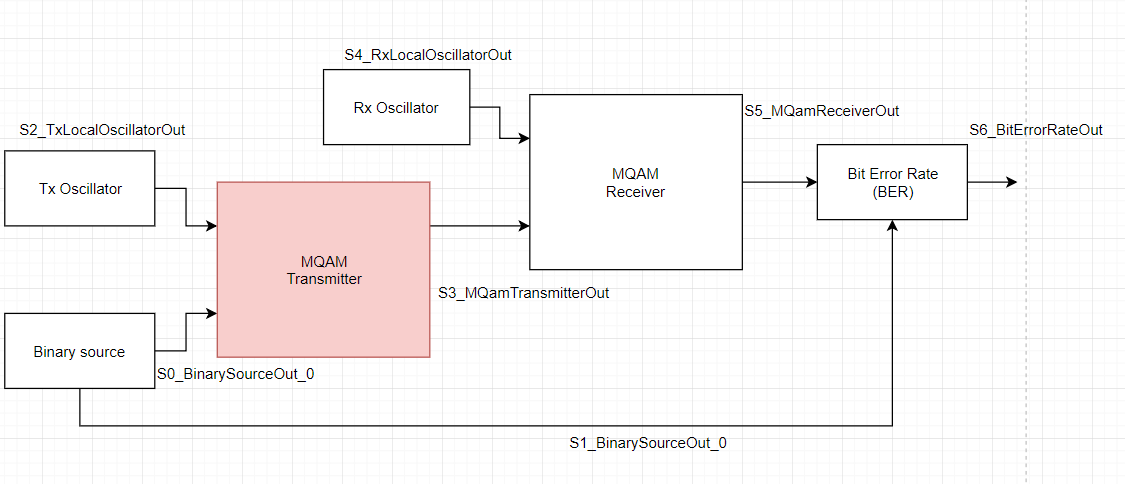
\includegraphics[scale=0.75]{./lib/m_qam_transmitter/figure_PLoureiro/MQAM_Transmitter_0.png}
	\caption{Block diagram of a transmission system}\label{MQAM_transmitter_block_diagram_simple}
\end{figure}

\subsection*{Functional description}
This block starts with a MQAM Mapper. In case of QPSK (M=4) the MQAM Mapper gives a point in the I-Q space per 2 bits received. The next two blocks are Discrete to Continuous Time and Pulse Shaper. The Pulse Shaper block applies an electrical filter to the signal, the type of filter could be Raised Cosine, Gaussian, Square, Root Raised Cosine. This block ends with the IQ Modulator, which takes the amplitude and phase of the signal and generates a complex optical signal. Figure \ref{MQAM_transmitter_block_diagram}

\begin{figure}[H]
	\centering
	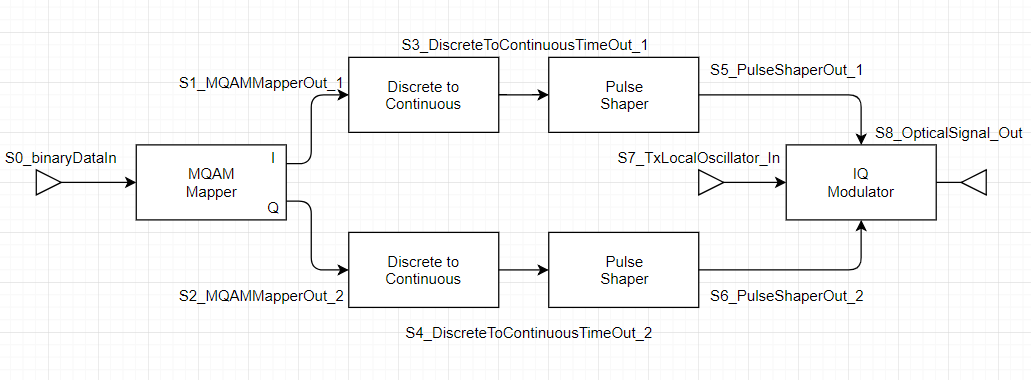
\includegraphics[width=\textwidth]{./lib/m_qam_transmitter/figure_PLoureiro/MQAM_Transmitter}
	\caption{Schematic representation of the block MQAM transmitter.}\label{MQAM_transmitter_block_diagram}
\end{figure}

\subsection*{Input parameters}

This block has a special set of functions that allows the user to change the basic configuration of the transmitter. The list of input parameters are summarized in table \ref{table}.

\begin{table}[H]
	\centering
	\begin{tabular}{|c|c|c|c|cccc}
		\cline{1-4}
		\textbf{Parameter} & \textbf{Type} & \textbf{Values} &   \textbf{Default}& \\ \cline{1-4}
        signalsFolderName & string & any & signals/SuperBlock\\
        & & &\_MQamTransmitter \\ \cline{1-4}
        logValue & bool & any & true \\ \cline{1-4}
        logFileName & string & any & SuperBlock\_\\
        & & & \_MQamTransmitter.txt \\ \cline{1-4}
		\multicolumn{4}{|c|}{ \textbf{MQAM Mapper} } \\ \cline{1-4}
		mValue & int & 2$^n$ & 4\\ \cline{1-4}
		iqAmplitudesValues & vector$<$\texttt{t\_complex}$>$ & any & \{ \{ 1, 1 \},\{ -1, 1 \},\\
        & & &\{ -1, -1 \},\{ 1, -1 \} \} \\ \cline{1-4}
		fTime & bool & any &  true\\ \cline{1-4}
		\multicolumn{4}{|c|}{ \textbf{Discrete To Continuous Time} } \\ \cline{1-4}
		nSamples & int & any & 8 \\
        PerSymbol & & & \\ \cline{1-4}
		\multicolumn{4}{|c|}{ \textbf{Pulse Shaper} } \\ \cline{1-4}
		impResponse & int & any & 16 \\
        TimeLength & & & \\ \cline{1-4}
        fType   & pulse\_shapper\_filter\_type & any$^1$ & RaisedCosine \\ \cline{1-4}
        rOffFactor & double & $\in \left[0,1\right]$ & 0.9 \\ \cline{1-4}
        pWidth & double & any & 5*10$^{-10}$ \\ \cline{1-4}
        pFilterMode & bool & any & false \\ \cline{1-4}
	\end{tabular}
	\caption{Binary source input parameters}
	\label{table}
\end{table}
$^1$ Raised Cosine, Gaussian, Square, Root Raised Cosine

\subsection*{Methods}

    \begin{enumerate}
         \item Block Declaration and Initialization
             \begin{itemize}
                 \item MQamTransmitter(initializer\_list$<$Signal *$>$ \&inputSig, initializer\_list$<$Signal *$>$ \&outputSig)
                 \item void initialize(void)
	             \item bool runBlock(void)
             \end{itemize}
         \item Functions to set parameters
             \begin{itemize}
                \item void setIqAmplitudes(vector<vector<t\_real>> iqAmplitudesValues)
                \item void setM(int mValue)
                \item void setFirstTime(bool fTime)
                \item void setNumberOfSamplesPerSymbol(int nSamplesPerSymbol)
                \item void setImpulseResponseTimeLength\_symbolPeriods\newline(int impResponseTimeLength)
                \item void setFilterType(pulse\_shapper\_filter\_type fType)
                \item void setRollOffFactor(double rOffFactor)
                \item void setPulseWidth(double pWidth)
                \item void setPassiveFilterMode(bool pFilterMode)
             \end{itemize}
         \item Functions to get parameters
             \begin{itemize}
                \item bool getFirstTime()
                \item int const getNumberOfSamplesPerSymbol(void)
                \item int const getImpulseResponseTimeLength\_symbolPeriods(void)
                \item pulse\_shapper\_filter\_type const getFilterType(void)
                \item double const getRollOffFactor()
                \item double const getPulseWidth()
                \item bool const getPassiveFilterMode()
             \end{itemize}
     \end{enumerate}
\subsection*{Input Signals}

\subparagraph*{Number:} 2

\subparagraph*{Type:} One optical signal from the local oscillator - S2\_TxLocalOscillatorOut \par
One binary from the binary source - S0\_BinarySourceOut\_0

\subsection*{Output Signals}

\subparagraph*{Number:} 1 optical

\subparagraph*{Type:} Optical signal - S3\_MQamTransmitterOut

\subsection*{Example}

\subsubsection*{Cardinality of the constellation}
In order to test the impact of the Cardinality of the constellation, the BER's of QPSK (4QAM) and of 16QAM will be analysed. The constellations are shown in the figures \ref{Constellation}.
\begin{figure}[H]
	\centering
        \begin{subfigure}{.55\textwidth}
        \centering
        	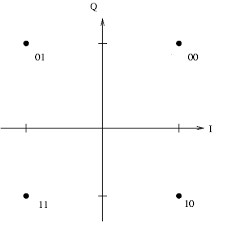
\includegraphics[scale=1]{./lib/m_qam_transmitter/figure_PLoureiro/4QAM_gray.png}
        \label{Example_4QAM_cons}\caption{Constellation of 4QAM}
        \end{subfigure}%
        \begin{subfigure}{.55\textwidth}
        \centering
        	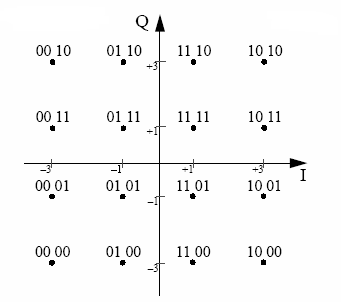
\includegraphics[scale=0.8]{./lib/m_qam_transmitter/figure_PLoureiro/16QAM_cons.png}
        	\caption{Constellation of 16QAM}\label{Example_16QAM_cons}
        \end{subfigure}
        \caption{}\label{Constellation}
\end{figure}
\begin{equation*}
BER 4QAM = 0
\end{equation*}
\begin{equation*}
BER 16QAM = 0.497487
\end{equation*}

As can be seen from the contents represented by the previous figure, 16QAM has 4 different amplitudes whereas 4QAM has only 2 different amplitudes.  It was noted also that the BER of 16QAM constellation is superior to 4QAM due to the fact that the 16QAM constellation has symbols which are surrounded by neighboring symbols, being much more subject to errors, although with the same noise.
\newpage
\subsubsection*{Constellation coding}
With the objective to analyze the impact of the constellation coding, the BER's will be tested with gray and without gray, the constellations are in the figures \ref{Constellation coding}.
\begin{figure}[H]
	\centering
        \begin{subfigure}{.55\textwidth}
        \centering
        	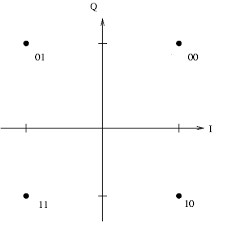
\includegraphics[scale=1]{./lib/m_qam_transmitter/figure_PLoureiro/4QAM_gray.png}
        \label{Example_4QAM_gray}\caption{Constellation of 4QAM with gray coding}
        \end{subfigure}%
        \begin{subfigure}{.55\textwidth}
        \centering
        	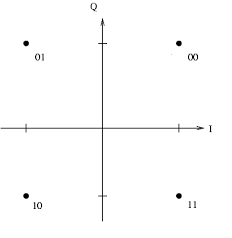
\includegraphics[scale=1]{./lib/m_qam_transmitter/figure_PLoureiro/4QAM_cons.png}
        	\caption{Constellation of 4QAM without gray coding}\label{Example_4QAM_nogray}
        \end{subfigure}
        \caption{}\label{Constellation coding}
\end{figure}
\begin{equation*}
BER 4QAM gray = 0
\end{equation*}
\begin{equation*}
BER 4QAM without gray = 0.247881
\end{equation*}

The BER of codification with gray is lower than without gray, because in gray codification the neighboring symbols only have 1 different bit while the codification without gray has neighboring symbols with 2 different bits. So, in the case of a wrong symbol, could have two wrong bits.

 \subsubsection*{Pulse shape}
 In this example was considered that the Pulse shaper and the electrical filter of the receiver has the same filter type.
 \begin{figure}[H]
	\centering
        \begin{subfigure}{.55\textwidth}
        \centering
        	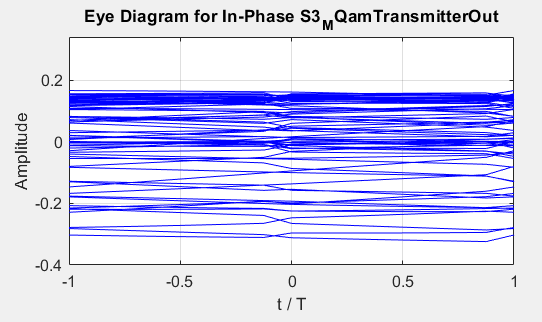
\includegraphics[scale=0.55]{./lib/m_qam_transmitter/figure_PLoureiro/16QAM_Gaussian_in.png}
        \label{Example_Gaussian_in}\caption{Eye diagram 16QAM transmission with fType=Gaussian }
        \end{subfigure}%
        \begin{subfigure}{.55\textwidth}
        \centering
        	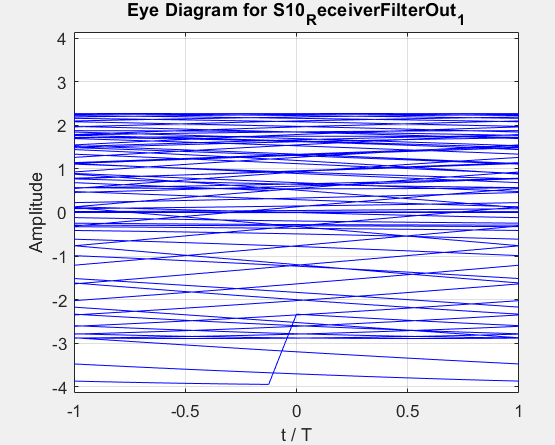
\includegraphics[scale=0.45]{./lib/m_qam_transmitter/figure_PLoureiro/16QAM_Gaussian_out.png}
        	\caption{Eye diagram 16QAM reception with fType=Gaussian }\label{Example_Gaussian_out}
        \end{subfigure}
        \caption{}\label{Gaussian}
\end{figure}

\begin{figure}[H]
	\centering
        \begin{subfigure}{.55\textwidth}
        \centering
        	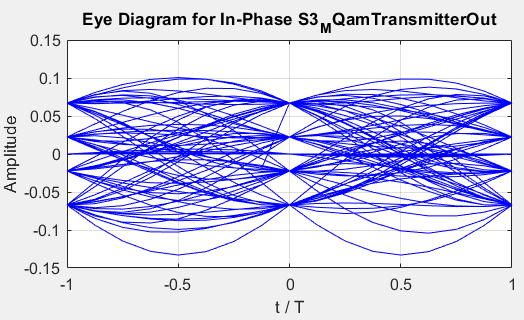
\includegraphics[scale=0.55]{./lib/m_qam_transmitter/figure_PLoureiro/16QAM_RaisedCosine_in.png}
        \label{Example_RaisedCoisine_in}\caption{Eye diagram 16QAM transmission with fType=RaisedCosine }
        \end{subfigure}%
        \begin{subfigure}{.55\textwidth}
        \centering
        	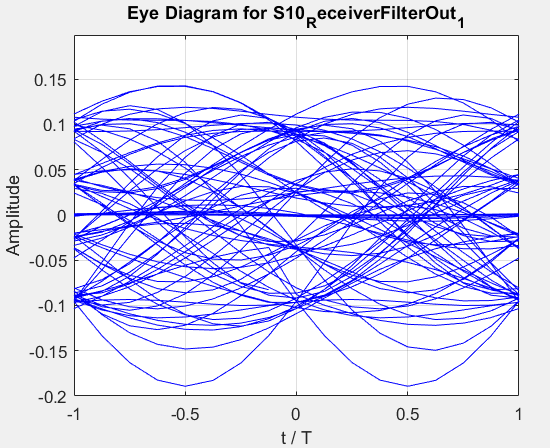
\includegraphics[scale=0.45]{./lib/m_qam_transmitter/figure_PLoureiro/16QAM_RaisedCosine_out.png}
        	\caption{Eye diagram 16QAM reception with fType=RaisedCosine }\label{Example_RaisedCoisine_out}
        \end{subfigure}
        \caption{}\label{RaisedCosine}
\end{figure}

\begin{figure}[H]
	\centering
        \begin{subfigure}{.55\textwidth}
        \centering
        	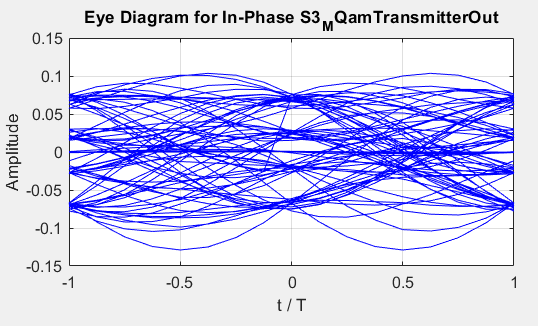
\includegraphics[scale=0.55]{./lib/m_qam_transmitter/figure_PLoureiro/16QAM_RootRaisedCosine_in.png}
        \label{Example_RootRaisedCoisine_in}\caption{Eye diagram 16QAM transmission with fType=RootRaisedCosine }
        \end{subfigure}%
        \begin{subfigure}{.55\textwidth}
        \centering
        	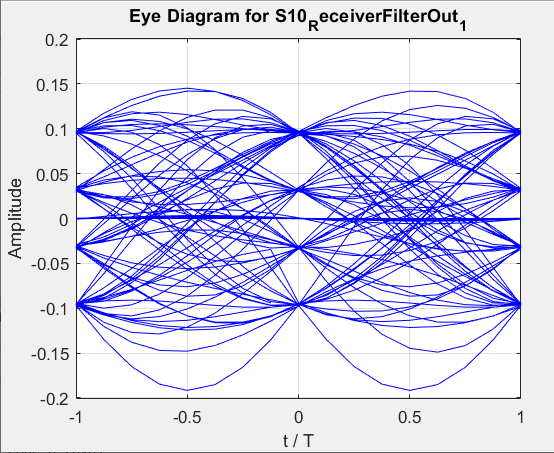
\includegraphics[scale=0.45]{./lib/m_qam_transmitter/figure_PLoureiro/16QAM_RootRaisedCosine_out.png}
        	\caption{Eye diagram 16QAM reception with fType=RootRaisedCosine}\label{Example_RootRaisedCoisine_out}
        \end{subfigure}
        \caption{}\label{RootRaisedCosine}
\end{figure}

By the figures \ref{Gaussian}, \ref{RaisedCosine} and \ref{RootRaisedCosine} the worst pulse shape was the Gaussian. The differences between the Root Raised Cosine and the Raised Cosine are that in the Raised Cosine the transmitter had Inter Symbol Interference (ISI) equal to 0, but in the receiver the ISI wasn't 0. The Root Raised Cosine had ISI equal to 0 in the receiver and different to 0 in the transmitter. The Square can´t be simulate because it gives an error whenever it compiles.

\subsection*{Open Issues}
\begin{enumerate}
    \item In the pulse shaper block, if the filter type is Square, it gives an error whenever it compiles.\par
    \item If we try to change the cardinality of the constellation to 16 doesn't happen nothing, the only way is to add a line for when the cardinality is 16.
\end{enumerate}

